\section{Probability Density}

For all \textit{continuous variables}, the probability mass function (pmf) is always equal to zero
\begin{align*}
  P(x) = 0 &\textnormal{ for all $x$}
\end{align*}
As a result, the pmf does not carry any information about a random variable. Rather, we can use the \textit{cumulative distribution function} (cdf) $F(x)$. In the continuous case, it equals
\begin{equation*}
  F(x) = \prob{X \leq x} = \prob{X < x}
\end{equation*}
These two expression for $F(x)$ differ by $\prob{X = x} = P(x) = 0$

In both continuous and discrete cases, the cdf $F(x)$ is a \textit{non-decreasing} function that \textit{ranges from 0 to 1}. In the discrete case, the graph of $F(x)$ has jumps of magnitude $P(x)$. For continuous distributions, $P(x) = 0$, which means no jumps. The cdf in this case is a continuous function.

Assume, additionally, that $F(x)$ has a derivative. This is the case for all commonly used continuous distributions, but in general, it is not guaranteed by continuity and monotonicity (the famous Cantor function is a counterexample).

\begin{definition}
  \textbf{Probability density function} (pdf, density) is the derivative of the cdf, $f(x) = F'(x)$. The distribution is called \textbf{continuous} if it has a density.
\end{definition}

Then, $F(x)$ is an antiderivative of a density. The integral of a density from $a$ to $b$ equals to the difference of antiderivatives, i.e.,
\begin{equation*}
  \int_a^b f(x)dx = F(b) - F(a) = \prob{a < X < b}
\end{equation*}
where we notice again that the probability in the right-hand side also equals $\prob{a \leq X < b}$, $\prob{a < X \leq b}$, and $\prob{a \leq X \leq b}$.

\begin{formula}{Probability density function}
  \noindent \begin{align*}
    f(x) &= F'(x)\\
    \prob{a < X < b} &= \int_a^b f(x)dx
  \end{align*}
\end{formula}

\begin{figure}[ht]
  \centering
  \includegraphics*[width=.5\textwidth]{img/Fig4.1.png}
  \caption{}
\end{figure}

Thus, probabilities can be calculated by integrating a density over the given sets. Furthermore, the integral $\int_a^b f(x)dx$ equals the area below the density curve between the points $a$ and $b$. Therefore, geometrically, probabilities are represented by areas (Figure 1). Substituting $a = -\infty$ and $b = +\infty$, we obtain
\begin{align*}
  &\int_{-\infty}^b f(x)dx = \prob{-\infty < X < b} = F(b)&\textnormal{ and }& &\int_{-\infty}^{+\infty} f(x)dx = \prob{-\infty < X < +\infty} = 1
\end{align*}
That is, the total area below the density curve equals 1.

Looking at Figure 1, we can see why $P(x) = 0$ for all continuous random variables. That is because
\begin{equation*}
  P(x) = \prob{x \leq X \leq x} = \int_x^x f = 0
\end{equation*}

Geometrically, it is the area below the density curve, where two sides of the region collapse into one.

\subsection{Analogy: pmf versus pdf}

\begin{table}[ht]
  \renewcommand{\arraystretch}{2}
  \centering
  \begin{tabular}{|l|l|l|} 
  \hline
  \textbf{Distribution}            & \textbf{Discrete}                               & \textbf{Continuous}                                 \\ 
  \hline
  Definition                       & $P(x) = \prob{X = x}$                           & $f(x) = F'(x)$                                      \\ 
  \hline
  Computing probabilities          & $\begin{aligned}\prob{X \in A} = \sum_{x \in A} P(x)\end{aligned}$          & $\begin{aligned}\prob{X \in A} = \int_A f(x)dx\end{aligned}$                    \\ 
  \hline
  Cumulative
  distribution
  function & $\begin{aligned}F(x) = \prob{X \leq x} = \sum_{y \leq x} P(y)\end{aligned}$ & $\begin{aligned}F(x) = \prob{X \leq x} = \int_{-\infty}^x f(y)dy\end{aligned}$  \\ 
  \hline
  Total probability                & $\begin{aligned}\sum_{x} P(x) = 1\end{aligned}$                             & $\begin{aligned}\int_{-\infty}^{+\infty} f(x)dx = 1\end{aligned}$                \\
  \hline
  \end{tabular}
  \caption{\textit{Pmf $P(x)$ versus pdf $f(x)$}}
\end{table}

The role of a density for continuous distributions is very similar to the role of the probability mass function for discrete distributions. Most vital concepts can be translated from the discrete case to the continuous case by replacing pmf $P(x)$ with pdf $f(x)$ and integrating instead of summing, as in Table 1.

\subsection{Joint and Marginal Densities}

\begin{definition}{}
  For a vector of random variables, the \textbf{joint cumulative distribution} function is defined as
  \begin{equation*}
    F_{(X, Y)} (x, y) = \prob{X \leq x \cap Y \leq y}
  \end{equation*}
  The \textbf{joint density} is the mixed derivative of the joint cdf,
  \begin{equation*}
    f_{(X, Y)} (x, y) = \frac{\partial^2}{\partial x \partial y} F_{(X, Y)} (x, y)
  \end{equation*}
\end{definition}

Similarly to the discrete case, a marginal density of $X$ or $Y$ can be obtained by integrating out the other variable. Variables $X$ and $Y$ are \textit{\textbf{independent}} if their \textit{joint density factors into the product of marginal densities}. Probabilities about $X$ and $Y$ can be computed by integrating the joint density over the corresponding set of vector values $(x, y) \in \mathbb{R}^2$. This is also analogous to the discrete case; see Table 2.

\begin{table}[ht]
  \renewcommand{\arraystretch}{2}
  \centering
  \begin{tabular}{|l|l|l|} 
  \hline
  \textbf{Distribution}                   & \textbf{Discrete}                                           & \textbf{Continuous}                                             \\ 
  \hline
  \multirow{2}{*}{Marginal
  Distributions} & $\begin{aligned}P(x) = \sum_y P(x, Y)\end{aligned}$                                     & $\begin{aligned}f(x) = \int f(x, y)dy\end{aligned}$                                         \\
                                          & $\begin{aligned}P(y) = \sum_x P(x, Y)\end{aligned}$                                     & $\begin{aligned}f(y) = \int f(x, y)dx\end{aligned}$                                         \\ 
  \hline
  Independence                            & $P(x, y) = P(x)P(y)$                                        & $f(x, y) = f(x) f(y)$                                           \\ 
  \hline
  Computing
  Probabilities                 & $\begin{aligned}\prob{(X, Y) \in A } = \mathop{\sum\sum}_{(x, y) \in A} P(x, y)\end{aligned}$ & $\begin{aligned}\prob{(X, Y) \in A} = \int \int_{(x, y) \in A} f(x, y) dx dy\end{aligned}$  \\
  \hline
  \end{tabular}
  \caption{\textit{Joint and marginal distributions in discrete and continuous cases.}}
\end{table}

\subsection{Expectation and Variance}

Continuing our analogy with the discrete case, \textit{expectation} of a continuous variable is also defined as a center of gravity,
\begin{equation*}
  \mu = \mathbf{E}(X) = \int xf(x)dx
\end{equation*}
This time, if the entire region below the density curve is cut from a piece of wood, then it will be balanced at a point with coordinate $\mathbf{E}(X)$, as shown in Figure 2.

\begin{figure}[ht]
  \centering
  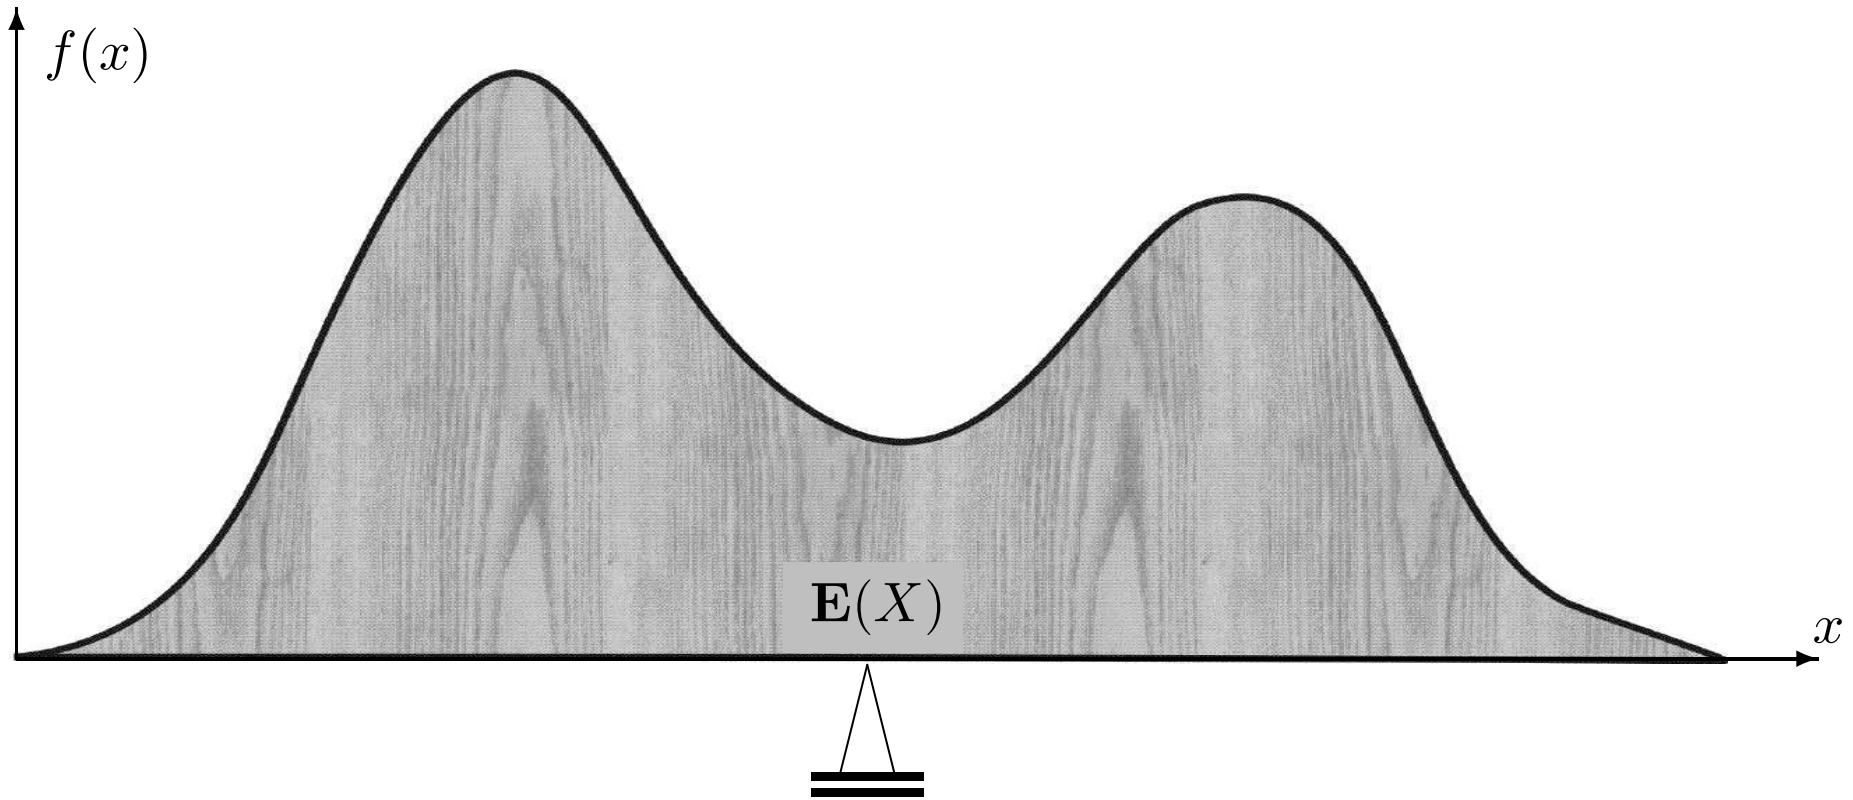
\includegraphics[width=.5\textwidth]{img/Fig4.3.png}
  \caption{\textit{Expectation of a continuous variable as a center of gravity.}}
\end{figure}

\textit{Variance, standard deviation, covariance}, and \textit{correlation} of continuous variables are defined similarly to the discrete case, see Table 3. All the properties in discrete cases extend to the continuous distributions. In calculations, don't forget to replace a pmf with a pdf, and a summation with an integral.

\begin{table}
  \renewcommand{\arraystretch}{2}
  \centering
  \begin{tabular}{|l|l|} 
  \hline
  \textbf{Discrete}                                   & \textbf{Continuous}                                  \\ 
  \hline
  $\begin{aligned}\mathbf{E}(X) = \sum_x xP(x)\end{aligned}$                      & $\begin{aligned}\mathbf{E}(X) = \int xf(x)dx\end{aligned}$                       \\ 
  \hline
  % Second Row
  $\begin{aligned}\text{Var}(X) &= \mathbf{E}(X - \mu)^2\\
                                &= \sum_x (x - \mu)^2 P(x)\\
                                &= \sum_x x^2 P(x) - \mu^2\\
  \end{aligned}$ 
  & 
  $\begin{aligned}\text{Var}(X) &= \mathbf{E}(X - \mu)^2\\
                                &= \int (x - \mu)^2 f(x)dx\\
                                &= \int x^2 f(x)dx - \mu^2    
  \end{aligned}$\\
  \hline

  %Third Row
  $\begin{aligned}\text{Cov}(X, Y) &= \mathbf{E}(X - \mu_X)(Y-\mu_Y)\\
                                   &= \sum_x \sum_y (x - \mu_X)(y - \mu_Y)P(x, y)\\
                                   &= \sum_x \sum_y (xy)P(x, y) - \mu_X \mu_Y
  \end{aligned}$
  &
  $\begin{aligned}\text{Cov}(X, Y) &= \mathbf{E}(X - \mu_X)(Y-\mu_Y)\\
                                   &= \int \int (x - \mu_X)(y - \mu_Y)f(x, y)dxdy\\
                                   &= \int \int (xy)f(x, y)dxdy - \mu_X \mu_Y
  \end{aligned}$\\
  \hline
  \end{tabular}
  \caption{\textit{Moments for discrete and continuous distributions.}}
\end{table}

\begin{example_break}{}
  The lifetime, in years, of some electronic component is a continuous random variable with the density
  \begin{equation*}
    f(x) = \begin{cases}
      \dfrac{k}{x^3} &\textnormal{ for } x \geq 1\\
      0 &\textnormal{ for } x < 1\\
    \end{cases}
  \end{equation*}
  Find $k$, draw a graph of the cdf $F(x)$, and compute the probability for the lifetime to exceed 5 years. Then computer expectation and variance.

  Find $k$ from the condition $\begin{aligned}\int f(x)dx = 1\end{aligned}$:
  \begin{equation*}
    \int_{-\infty}^{+\infty} f(x)dx = \int_1^{+\infty} \frac{k}{x^3} dx = - \frac{k}{2x^2} \Big|_{x = 1}^{+\infty} = \frac{k}{2} = 1
  \end{equation*}
  Hence, $k = 2$. Integrating the density, we get the cdf,
  \begin{equation*}
    F(x) = \int_{-\infty}^x f(y)dy = \int_1^x \frac{2}{y^3} dy -\frac{1}{y^2} \Big|_{y=1}^x = 1 - \frac{1}{x^2}\ \ \ \ \textnormal{for $x > 1$}
  \end{equation*}
  
  Next, compute the probability for the lifetime to exceed 5 years,
  \begin{equation*}
    \prob{X > 5} = 1 - F(5) = 1 - \left(1 - \frac{1}{5^2}\right) = 0.04
  \end{equation*}
  We can also obtain this probability by integrating the density,
  \begin{equation*}
    \prob{X > 5} = \int_5^{+\infty} f(x)dx = \int_5^{+\infty} \frac{2}{x^3}dx = -\frac{1}{x^2} \Big|_{x = 5}^{+\infty} = \frac{1}{25} = 0.04
  \end{equation*}
  
  Its expectation equals
  \begin{equation*}
    \mu = \mathbf{E}(X) = \int x f(x)dx = \int_1^{\infty} 2x^{-2}dx = -2x^{-1} \Big|_1^{\infty} = 2
  \end{equation*}

  Computing its variance, we run into a ``surprise'': This variable does not have a finite variance!
  \begin{equation*}
    \sigma^2 = \text{Var}(X) = \int x^2 f(x)dx - \mu^2 = \int_1^{\infty} 2x^{-1}dx - 4 = 2 \ln x \Big|_1^{\infty} - 4 = +\infty
  \end{equation*}
\end{example_break}
